% !TeX encoding = UTF-8
% !TeX spellcheck = sk_SK
% !TeX root = ../main.tex
%\chapter{Knižnica Snap.svg.js}





\chapter{Learning Raphael JS Vector Graphics}
%V práci cituj: \cite{Dawber} , strany sa cituju takto: \cite[p.~215]{Dawber} \\ Priklady z knihy:\url{http://raphaeljsvectorgraphics.com/}  \cite{Dawber} .
%Z tejto knihy idem pridávať do bakalárky nasledovné veci:
%Namet na zmenu: pouzit to demo, ktore mi poslal veduci na transformaciu zmeny. 


\section{Porovnanie spôsobu vykreslenia cez \acs{SVG} \acs{SMIL} a Snap}

Kreslenie vektorov je jednoduchšie cez Snap ako čisto písanie SVG. 

Príklad kreslenia obdĺžníka a animovanie šírky z 50 pixlov na 100 pixelov cez SVG SMIL:\cite[p.~9]{Dawber}
\begin{lstlisting}
<svg>
<rect x="10" y="10" width="50" height="30">
<animate attributeType="XML"
attributeName="width"
to="100"
fill="freeze"
dur="10s"  />
</rect></svg>
\end{lstlisting}

Nakreslíme obdĺžnik na súradniciach (10, 10) s šírkou 50, a výškou 30 použitím elementu $<$rect$>$. Zoskupený element $<$animate$>$ definuje animáciu zmeny šírky obdĺžnika na šírku 100 px, ktorá trvá desať sekúnd. Kde fill="freeze" je použité na zachovanie stavu obdĺžnika po ukončení animácie. Inak by bola nastavená na 50. 

Ekvivalent k animácii cez Snap API v nasledujúcom príklade:

\begin{lstlisting}
paper = Snap();
var rect = paper.rect(10, 10, 50, 30);
rect.animate({
width: 100
}, 10000);
\end{lstlisting}

Syntax metód animate a rect je výstižnejšia a lepšia na pochopenie. Snap sa tiež dobre integruje s inými knižnicami, ako napríklad jQuery. 


%%%%%%%%%%%%%%%%%%%%%%%%%%%%%%%%%%%%%%%%%%%%%%%%%%%%%%%%%%%%%%%%%%%%%%%%%%%%%%%%%%%%%%%%%%%%%%%%%%%%%%%%%%%%%%%%%%%%%%%%%%%%%%%%%%%%%%%%%%%%%%%%%%%%%%%%%%%%%%%%%%%%%%%%%%%%%%%%%%%%%%%%%%%%%%%%%%%%%%%%%%%%%%%%%%
\newpage
%Jednoduche kreslenie ,
%Interakcia ,
%Animovanie.. 
%
%Krok 0: ziskanie Snapu...


\section{Krok 1: Inicializácia plátna na kreslenie}
%viewport = výrez
Na to, aby sme boli schopní kresliť grafické komponenty, tak potrebujeme definovať miesto, kde budú vykreslené. 
%Určenie miesta, kde bude vykreslené plátno je buď viditeľné okno vo webovom prehliadači, alebo viewport. 
Viditeľná oblasť okna prehliadača, alebo viewport, definuje oblasť, v ktorej sa vykreslí komponent na plátno.
SVG špecifikácia referuje ako miesto vykreslenia seba ako viewport. 
Inak povedané viewport je akákoľvek obdĺžniková oblasť.
Okno prehliadača je referencia na viewport a kresliaca oblasť je plátno.   \cite{Dawber}


Vytvorenie plátna cez Snap konštruktor sa dá urobiť viacerými spôsobmi.

\subsection{Súradnice plátna}

TODO Na to, aby bolo plátno responzívne vo webovom prehliadači musí byť nastavené tieto dve veci: 
 \begin{itemize}
 	\item definovaný viewBox
 	\item výška a šírka plátna musí byť v relatívnych rozmeroch, najlepšie nastavená na 100\%
 \end{itemize}
 %var s = Snap("$ #s $vgout"); 
 %s.attr({ viewBox: "0 0 600 600" });
 %2. sposob pri definicii svg $ <svg id="idsvg" viewBox="0 0 600 600" weight="100\%" height="100\%"> $

Nasledujúci príkaz zadefinuje pláno s rozmermi šírka je 300 a výška 200. 
\begin{lstlisting}
var paper = Snap(300, 200);
\end{lstlisting}


Na obrázku \ref{fig:suradnice1}  je znázornená východzí súradnicový systém plátna vytvoreného cez Snap konštruktor. 
Začiatok súradnic na osi x, y je rovné nule. Bod na plátne so súradnicami x = 300, y = 200 alebo (300, 200) vo vektorovom zápisu je bod 300px vpravo od začiatku x-ovej osi a 200px dole od počiatku y-ovej osi. 

\begin{center}
	\begin{figure}[H]
		\centering
		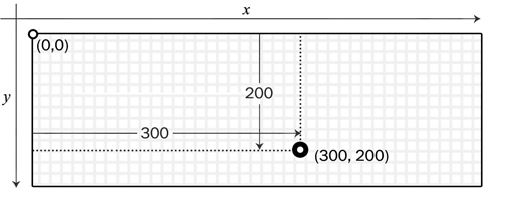
\includegraphics[width=0.5\linewidth]{obrazky/suradnice1}
		\caption{Súradnicový systém plátna s bodom (300, 200)}
		\label{fig:suradnice1}
	\end{figure}
\end{center}

\subsection{DOM element}

Dosť často je potrebné použiť existujúci DOM element ako kontajner pre plátno než viewport. Ako element môžeme použiť napríklad:
\begin{lstlisting}
<div id="mojePlatno"></div>  
\end{lstlisting}

Nasledujúcim kódom vytvorím 500px široké a 300px vysoké plátno.

\begin{lstlisting}
var paper = Snap("mojePlatno", 500, 300);
\end{lstlisting}

Keď využívam túto formu konštruktora, tak prvý element je ID elementu. Alternatívne sa dá prvý parameter DOM element napísať nasledovným spôsobom: 
\begin{lstlisting}
Snap(document.getElementById('mojePlatno'), 500, 300);
\end{lstlisting}



\subsubsection{\acs*{SVG} v HTML dokumente}

SVG môže byť zobrazená buď ako inline v HTML dokumente, alebo ako vloženým samostatného .SVG súboru. 
V tabuľke \ref{vytvorenie:SVG} sú vymenované HTML tagy na zobrazenie SVG. 


\begin{table}[H]
	\begin{center}
		\begin{tabular}{|l|l|}
			\hline \textbf{Technika} & \textbf{Popis} \\ 
			\hline
			\hline $<$embed$>$ tag & Načíta vytvorený SVG súbor.  \\ 
			\hline $<$object$>$ tag & Nepovoľuje skriptovanie.  \\ 
			\hline $<$iframe$>$ tag & Zobrazí SVG v rámci  \\ 
			\hline Inline $<$svg$>$ tag & Vytvorí Svg  \\ 
			\hline 
		\end{tabular} 
	\end{center}
	\caption{Spôsoby vytvorenia SVG v HTML dokumente}
	\label{vytvorenie:SVG}
\end{table}


%Príklady načítania SVG v HTML dokumente:
%\begin{itemize}
%\item Image 	
%\begin{lstlisting}
%<img src="stanica2.svg" width = "50" height= "50" />
%\end{lstlisting}
%\item Embed
%\begin{lstlisting}
%<embed src="stanica2.svg" width = "50" height= "50" />
%\end{lstlisting}
%\item Objekt
%\begin{lstlisting}
%<object type="image/svg+xml" data="stanica2.svg"
%width="50" height="50"></object>
%\end{lstlisting}
%\item IFrame
%\begin{lstlisting}
%<iframe src="stanica2.svg" width = "50" height= "50">
%</iframe>
%\end{lstlisting}
%\item Inline
%\begin{lstlisting}
%<svg width="100" height="100"> 
%<circle cx="50" cy="50" r="40"/> </svg>
%\end{lstlisting}
%	
%
%\end{itemize}





%%%%%%%%%%%%%%%%%%%%%%%%%%%%%%%%%%%%%%%%%%%%%%%%%%%%%%%%%%%%%%%%%%%%%%%%%%%%%%%%%%%%%%%%%%%%%%%%%%%%%%%%%%%%%%%%%%%%%%%%%%%%%%%%%%%%%%%%%%%%%%%%%%%%%%%%%%%%%%%%%%%%%%%%%%%%%%%%%%%%%%%%%%%%%%%%%%%%%%%%%%%%%%%%%%%%%%%%%
\newpage

\section{Kreslenie základných tvarov cez Snap API}

Snap API poskytuje metódy na kreslenie jednoduchých tvarov. 

\begin{table}[H]
	\begin{center}
		\begin{tabular}{|l|l|l|l|}
			\hline \textbf{Tvar} & \textbf{SVG element} & \textbf{Snap metoda} & \textbf{Atribúty} \\ 
			\hline
			\hline Obdlžnik & $<$rect$>$ & .rect() & x, y, šírka, výška, rx, ry \\ 
			\hline Kruh & $<$circle$>$ & .circle() & r, x, y, cx, cy, rx, ry \\ 
			\hline Elipsa & $<$ellipse $>$ & .ellipse() & x, y, cx, cy, rx, ry \\ 
			\hline Čiara & $<$line$>$ & .line() & x1, y1, x2, y2 \\ 
			\hline Polyline & $<$polyline$>$ & .polyline() & pole x, y suradnic bodov \\ 
			\hline Polygon & $<$polygon$>$ & .polygone() & pole x, y suradnic bodov \\ 
			\hline Path & $<$path$>$ & .path() & vid tabuľka \ref{prikazy:Path}  \\ 
			\hline 
		\end{tabular} 
		
	\end{center}
	
	\label{porovnanieSVG:Snap}
	\caption{Zoznam tvarov, ktoré podporuje SVG a Snap API, a TODO TODO POROZMYSLAT NAD NAZVOM a atributy pre definovanie tvaru}
\end{table}




Tvar, ktorý je vykreslený cez Snap API má nasledovnú syntax: 

\begin{lstlisting}
var paper = Snap(...);
var tvar = paper.NazovSnapMetody({
nazovAtributu: "hodnotaAtributu",
...
});
\end{lstlisting}

Tvar, ktorý je vykreslený priamo na HTML webovej stránke má vo vnútri elementu $<$svg$>$ definované atribúty nasledujúcim spôsobom: 

\begin{lstlisting}
<ElementTvar nazovAtributu = "hodnotaAtributu" ... />
\end{lstlisting}


\subsection{Popis atribútov tvarov}

Názvy atribútov a ich význam pre obdĺžnik, kruh, elipsu sú vyjadrené v tabuľke \ref{parametre:tvar} 

\begin{table}[H]
	\begin{center}
		\begin{tabular}{|l|l|}
			\hline \textbf{Parameter} & \textbf{Poznámka} \\ 
			\hline
			\hline x, y & súradnica x-osi, y-osi  \\ 
			
			\hline cx & x-os súradnica centra kruhu, alebo elipsy \\ 
			\hline cy & y-os súradnica centra kruhu, alebo elipsy \\ 
			\hline r & polomer kruhu, elipsy alebo okruhlých rohov na obdĺžniku \\ 
			\hline rx & horizontálny polomer elipsy \\ 
			\hline ry & vertikálny polomer elipsy \\ 
			\hline x1, y1 & začiatočné x, y súradnice \\
			\hline x2, y2 & konečné x, y súradnice \\
			
			%\hline width, height & šírka, výška\\
			\hline
		\end{tabular} 
		
	\end{center}
	\caption{Názvy atribútov a ich význam}
	\label{parametre:tvar}
\end{table}

Pre útvary polyline, polygon sú atribúty dvojice súradníc osi x, y, ktoré určujú body, ktoré sa spoja. 



\subsubsection{Path tvar}


V Snap API je to metóda Paper.path([pathString]), ktorá vytvorí $<$path$>$ element podľa daného reťazca.  Parameter pathString pozostáva reťazca skladajúceho sa z jedno písmenkových príkazov, nasledovanými bodkami a oddeľovaný argumentami a číslami. Príkazy sú uvedené v tabuľke \ref{prikazy:Path}.

Napríklad: "M10,20L30,40" - obsahuje príkazy: M s argumentami (10, 20) a L (30, 40). Rozdiel vo veľkosti písma vyjadruje to, či ide o absolútnu, alebo relatívnu cestu. Ak sú malé znaky jedná sa o relatívne, v prípade veľkých znakov absolútna cesta. 


\begin{center}
	\begin{table}[H]
		\begin{center}
			\begin{tabular}{|c|l|c|}
				\hline \textbf{Príkaz} & \textbf{Názov} & \textbf{Parametre} \\
				\hline
				\hline M & moveto & (x y)+ \\ 
				\hline Z & closepath & (none) \\ 
				\hline L & lineto & (x y)+ \\ 
				\hline H & horizonal lineto & x+ \\ 
				\hline V & vertical lineto & y+ \\ 
				\hline C & curveto & (x1 y1 x2 y2 x y)+ \\ 
				\hline S & smooth curveto & (x2 y2 x y)+ \\ 
				\hline Q & quadratic Bézier curveto & (x1 y1 x y)+ \\ 
				\hline T & smooth quadratic Bézier curveto & (x y)+ \\ 
				\hline 
			\end{tabular} 
		\end{center}
		\caption{Niekoľko príkazov na tvorbu Path elementu}
		\label{prikazy:Path}
	\end{table}
\end{center}


\section{Vykreslenie obrázku}
Snap povoľuje vloženie bitmapových obrázkov (.jpg alebo .png) na plátno. Používa metódu image z Paper objektu. Parametre metódy image sú: zdroj, x, y, šírka, výška. Príklad kódu, ktorý vkladá .jpg obrázok do plátna:
\begin{lstlisting}
var paper = Snap("mojePlatno", 300, 200);
paper.image("obrazok.jpg", 15, 15, 100, 150);
\end{lstlisting}


\section{Atribúty elementu}

Tvary, ktoré sa dajú nakresliť sa môžu vyfarbiť, orámovať alebo mnoho iných atribútov sa dá nastaviť. Keď sa vytvorí tvar, tak sa vráti Element objekt. Tento objekt má attr metódu, ktorá akceptuje key-value pár atribútov. V tomto odseku sa pozrieme na rôzne atribúty, ktoré môžu byť aplikované na naše grafické komponenty používajúc túto metódu. 

%Element.attr(...) vráti alebo nastaví dané atribúty elementu. Medzi parametre patrí buď objekt, ktorý sa skladá s páru kľúč-hodnota, alebo názvu atribútu. 

\subsection{Výplň elementu - fill }

Pozadie pre element nastavím cez metódu attr použitím fill atribútu ako parameter. Pre jednofarebné výplne je formát vyjadrený cez CSS špecifikáciu. CSS špecifikácia farieb je nasledovná: \#rrggbb alebo skrátene \#rgb , rgb(r, g, b) reťazec alebo slovne. 
Napríklad: 
\begin{lstlisting}
var kruh = paper.circle(50, 50, 40).attr("fill", "red");
\end{lstlisting}

Ďalšie spôsoby výplne elementu sú obrázkom,  gradientom, alebo vzorom. 
Pre nastavenie neprehľadnosti nastavíme atribút "fill-opacity" hodnotou čísla v rozsahu od 0-1. Element pri "fill-opacity": 1 je neprehľadný.  

\subsection{Nastavenie okraja elementu - stroke}

Elementy môžu mať niekoľko rôznych druhov okrajových atribútov. Prehľad tých najznámejších je v tabuľke \ref{parametre:styl}.\cite{styly}


\begin{table}[H]
	\begin{center}
		
		\begin{tabular}{|l|l|l|}
			\hline \textbf{Atribút pre attr() } &\textbf{CSS atribút} & \textbf{Poznámka} \\ 
			\hline 
			
			\hline stroke & stroke & farba výplne okraja \\ 
			\hline strokeWidth & stroke-width & šírka okraja v px, default je 1 \\ 
			\hline
			strokeOpacity & stroke-opacity & neprehľadnosť, 0-1 \\
			\hline strokeLinecap & stroke-linecap & ["butt", "square", "round"], tvar - okraj konca\\ 
			\hline strokeLinejoin & stroke-linejoin & ["bevel", "round", "miter"], tvar - okraj roku\\ 
			
			\hline strokeDasharray &stroke-dasharray & pole čiarok, bodiek.., napr.5,3,2\\
			
			\hline
		\end{tabular} 
	\end{center}
	\caption{Výber možných stroke atribútov}
	\label{parametre:styl}
\end{table}


\section{Zoskupovanie elementov}

Niekedy je potrebné použiť rovnaké atribúty, transformácie, alebo animácie pre viacero elementov. V Snap API je možné využiť metódu group alebo g. Group zoskupí viacero elementov do množiny. Príkazom add sa dajú pridať ďalšie prvky. V množine sa dajú meniť atribúty pre viacero prvkov naraz volaním metódy attr. 

Príklad zoskupenia elementov. Výsledné zoskupenie je zobrazené na obrázku \ref{fig:grupovanieElementov}. 

\begin{lstlisting}
var paper = Snap();
var kruh = paper.circle(50, 50, 40);
var obdlznik = paper.rect(120, 10, 80, 80);
var elipsa = paper.ellipse(270, 50, 40, 20);

var group = paper.g(kruh, obdlznik);
group.add(elipsa);

group.attr({
	fill: 'yellow',
	stroke: '#000',
	strokeWidth: 5, 
	strokeDasharray: [3, 5, 1]
});
\end{lstlisting}

\begin{figure}[H]
\centering
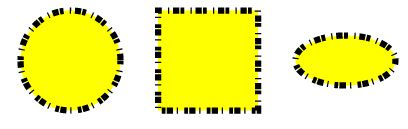
\includegraphics[width=0.7\linewidth]{obrazky/grupovanieElementov}
\caption{Príklad zoskupenia elementov a následná zmena atribútov}
\label{fig:grupovanieElementov}
\end{figure}








%
%
%\newpage
%\clearpage
%TOTO BUDE PRIKLAD KED BUDEM MAT UZ NAPISANE ATTRIBUTY NA ZMENU STYLU
%asi by bolo velmi vhodne pouzit nejake ine demo, ako ubohy kruh, teda asi teplomer, alebo mapu, ale urcite nieco ine ako kruh!!!!!!!!!!
%
%\subsubsection{PRIKLAD TVORBY KRUHU A NASTAVENIE ATRIBUTOV }
%
%Kód vytvoreného kruhu: 
%
%\begin{lstlisting}
%<svg width="100" height="100">
%<circle cx="50" cy="50" r="40" stroke="black" stroke-width="2" fill="silver" />
%</svg>	
%\end{lstlisting}
%
%SVG obrázok začína s $<$svg$>$ elementom. Atribúty elementu $<$svg$>$ sú width a height. Definujú šírku a výšku SVG obrázka. Element $<$circle$>$ je použitý na nakreslenie kruhu.
%
%
%TODO TODO TODO
%
%Atribúty stroke a stroke-width určujú to ako bude vyzerať obrys útvaru. Kruh má nastavený 2px čierny okraj. 
%Atribút fill vyplní vnútro kruhu. V príklade je vyplnený sivou farbou. Tag, ktorý uzavrie SVG obrázok je $<$$/$svg$>$. Keďže SVG je validné XML, tak všetky elementy musia byť správne zatvorené. \cite{inline}
%
%Kruh vytvorený cez Snap API má nasledovný kód:
%
%\begin{lstlisting}
%var paper = Snap(100, 100);
%var kruh = paper.circle(50, 50, 40);
%kruh.attr({
%stroke: "black", 
%strokeWidth: 2, 
%fill: "silver"
%});
%
%\end{lstlisting}
%
%
%Vykreslí sa na HTML stránku obrázok \ref{jednoduchyKruh}. Obidva spôsoby vykreslili kruh na webovej stránke úplne rovnako.  
%
%\begin{figure}[hp]
%	\begin{center}
%		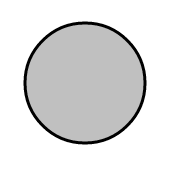
\includegraphics  {obrazky/jednoduchyKruh.png}
%		\caption{Vykreslený kruh vytvorený cez SVG, a Snap API}
%		\label{jednoduchyKruh}
%	\end{center}
%\end{figure}
%
%

\subsection{Maskovanie - Element.mask()}
TODO - 
PRE DANY ELEMENT VOLAM FUNKCIU ATTR, KDE NASTAVIM VLASTNOST MASK 
NAPR. mask: ellipse

/ Now more interesting stuff
// Let's assign this group as a mask for our big circle
bigCircle.attr({
	mask: discs
});

\section{Práca s textom - Paper.text(x, y, text)}

Vykreslenie textu na plátne namiesto HTML markup s CSS štýlovaným umožňuje animovať a transformovať v rovnakým spôsobom ako iné tvary. Text vytvorení cez metódu text. Parametre metódy text sú súradnice x, y a text, ktorý sa vykreslí. Vlastnosti textu sa dajú zmeniť volaním metódy attr. V tabuľke sú atribúty, ktoré sa dajú zmeniť prostredníctvom metódy attr. 


\begin{table}[H]
	
	\begin{center}
		
		\begin{tabular}{|l|l|p{8cm}|}
			\hline \textbf{Snap atribút}  &\textbf{ CSS atribút}  & \textbf{Poznámka} \\ 
						\hline
			\hline font & font & napr. "30px Helvetica, sans-serif",\\ 
			\hline textAnchor & text-anchor & pozícia textu, napr. "middle" \\ 
			\hline fill & fill & výplň textu farbou, gradientom, vzorom \\ 
			\hline fontSize  & font-size  & veľkosť textu  \\ 
			\hline fontFamily & font-family & napr. "monospace" \\ 
			\hline fontStyle & font-style  & štýl písma, napr. kurzíva  \\ 
			\hline fontVariant  & font-variant  & napr. "small-caps"  \\ 
			\hline  fontWeight & font-weight  &  hrúbka písma,  napr. normal, bold, bolder, lighter, 100-900\\ 
			\hline 
		
		\end{tabular} 
		
		
	\end{center}
\label{tab:text}
\caption{Atribúty na zmenu vlastností elementu text}
\end{table}

Príklad zmeny farby: 
\begin{lstlisting}
var paper = Snap();
var text = paper.text(30, 100, "Namestovo");

text.attr({
	textAnchor: "middle",
	fill: "#00b", 
	fontSize: '16px', 
	fontFamily: "Veranda", 
	fontStyle: "italic", 
	fontVariant: "small-caps", 
	fontWeight: 800, 
});
\end{lstlisting}

Na obrázku \ref{fig:textPriklad} je zobrazený text, ktorý bol uvedený v príklade. 

\begin{figure}[H]
\centering
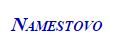
\includegraphics{obrazky/textPriklad}
\caption{Príklad na zmenu atribútov v texte.}
\label{fig:textPriklad}
\end{figure}



\section{Transformácie - Element.transform(...)}

Element.transform(\[tstr\])

r-30, 50, 10t10, 20s1.5
Adds transformation to the element which is separate to other attributes, i.e. translation doesn’t change x or y of the rectange. The format of transformation string is similar to the path string syntax:

"t100,100r30,100,100s2,2,100,100r45s1.5"
Each letter is a command. There are four commands: t is for translate, r is for rotate, s is for scale and m is for matrix.

There are also alternative “absolute” translation, rotation and scale: T, R and S. They will not take previous transformation into account. For example, ...T100,0 will always move element 100 px horisontally, while ...t100,0 could move it vertically if there is r90 before. Just compare results of r90t100,0 and r90T100,0.

So, the example line above could be read like “translate by 100, 100; rotate 30 stupnov around 100, 100; scale twice around 100, 100; rotate 45 stupnov around centre; scale 1.5 times relative to centre”. As you can see rotate and scale commands have origin coordinates as optional parameters, the default is the centre point of the element. Matrix accepts six parameters.

Usage
\begin{lstlisting}


var el = paper.rect(10, 20, 300, 200);
// translate 100, 100, rotate 45, translate -100, 0
el.transform("t100,100r45t-100,0");
// if you want you can append or prepend transformations
el.transform("...t50,50");
el.transform("s2...");
// or even wrap
el.transform("t50,50...t-50-50");
// to reset transformation call method with empty string
el.transform("");
// to get current value call it without parameters
console.log(el.transform());
\end{lstlisting}
%Parameters
%tstrstring
%transformation string
%If tstr isn’t specified
%
%Returns:stringcurrent transformation string
%
%else
%
%Returns:objectElement





Keď vytváram element v Snap, tak efektívne vytváram \ac{DOM} objekt. TODO... \cite [page~51] {Dawber} 

\subsection{Suradnicovy system}

\subsection{Jednoduché transformácie}

Basic transformations and event
handling
We perform transformations in Raphaël using the transform method on elements,
which accepts as an argument a transformation string. Transformation strings define
a sequence of transformations to take place on a particular element.

You can also transform elements and sets using the transform attribute. This is often
convenient when we are changing multiple attributes at the same time. You will see
examples of this in Chapter 5, Vector Animation.
Basic transformations
Like a path string, a transformation string is composed of a number of commands
defined in the order in which they are to be interpreted. The syntax for the basic
commands is as follows, where brackets indicate optional parameters: \ref{tab:trasf}

\begin{table}[H]

\begin{center}
	
\begin{tabular}{|c|c|c|}
	\hline \textbf{Príkaz} & \textbf{Parameter} & \textbf{Príklad} \\ 
	\hline T, t & x, y & t50,100 \\ 
	\hline R, r & uhol, (bod rotacie x, y) & r45,0,0 \\ 
	\hline S, s & scale x, y, (scale bod x, y) & S 2,4.5,75,125 \\ 
	\hline 
\end{tabular} 	
\end{center}
\label{tab:trasf}
\caption{Jednoduché príkazy na vytvorenie parametra stringu pre metodu v Element.transform(...) TODO}

\end{table}

As with a path string, transformation strings have uppercase and lowercase
variants. The uppercase variant means that we transform, irrespective of the
previous transformation, while the lowercase variant takes previous transformations
into account. The following examples demonstrate the basic transformations.\cite[p.~52]{Dawber}

V tabulke \ref{tab:svgTrans} je prehlad transfoormacii umoznujuce pre SVG. TODO \cite[p~73]{Eisenberg}

\url{http://commons.oreilly.com/wiki/index.php/SVG_Essentials/Transforming_the_Coordinate_System}

\begin{table}[H]
	\begin{center}
	\begin{tabular}{|l|p{9cm}|}
	\hline \textbf{Transformation} & \textbf{Popis} \\ 
	\hline translate(x,y) & Posunie súradnicový systém na dané x, y.  \\ 
	\hline scale(xFactor, yFactor) & Vynasobí súradnice o daný násobok. Násobok môže byť aj zlomok, záporné číslo \\ 
	\hline rotate(uhol) & Zrotuje súradnice o daný uhol. Stred rotácie je (0,0).  \\ 
	\hline rotate(uhol, centerX, centerY) & Zrotuje súradnice o daný uhol, s danými súradnicami stredu rotácie.  \\ 
	\hline skewX(uhol) & Nakloní všetky x-ové súradnice v danom uhle.  \\ 
	\hline skewY(uhol) & Nakloní všetky y-ové súradnice v danom uhle.  \\ 
	\hline 
\end{tabular} 

\end{center}
\label{tab:svgTrans}
\caption{SVG transformácie }
\end{table}

TODO / TOTO JE Z JEDNEJ BAKALARKY O SVG .. 

Všetky transformácie grafických prvkov sa realizujú pridaním požadovanej transformácie do atribútu "transform". Keď sa teda v zdrojovom kóde uvádza, že bol zmenený súradnicový systém vo vnútri nejakej skupiny g pridaním atribútu transform = "scale (2)", tak môžeme vyjadriť túto zmenu vetou: "Všetky prvky vo vnútri danej skupiny boli zväčšené 2x."
Hodnotou atribútu transform je zoznam transformácií, z čoho vyplýva, že na ľubovoľný objekt možno súčasne aplikovať viac ako jednu transformáciu. Jednotlivé položky môžu byť oddelené medzerou alebo čiarkou.
Matrix (a, b, c, d, e, f) - všeobecná transformačné matice

Translate (tx, ty) - translácie alias posun. Všeobecný zápis: 'matrix (1 0 0 1 tx ty)'

Scale (sx, sy) - zmena mierky, ak je uvedená len jedna hodnota, prehliadač predpokladá, že obidve hodnoty sú rovnaké. Všeobecný zápis: 'matrix (sx 0 0 sy 0 0)'

Rotate (uhoľ [stred-x stred-y]) - rotácia, otáčanie o zadaný uhol okolo ľubovoľného stredového bodu otáčania [súradnice v hranatých zátvorkách nemusia byť uvedené, potom sú ich predvolené hodnoty 0,0]. Všeobecne (so stredom rotácie v 0,0) možno zapísať ako 'matrix (cos (uhoľ) sin (uhoľ)-sin (uhoľ) cos (uhoľ) 0 0)'

SkewX (uhoľ) - skosenie pozdĺž osi X. Všeobecný zápis: 'matrix (1 0 tan (uhoľ) 1 0 0)'

SkewY (uhoľ) - skosenie pozdĺž osi Y. Všeobecný zápis: 'matrix (1 tan (uhoľ) 0 1 0 0)'

\begin{lstlisting}
<animateTransform 
	attributeName="transform"
	 type="rotate" 
	 values="0;360;0" 
	 begin="2s" dur="4s"/>
\end{lstlisting}

\subsubsection{Translation}

Element.transform("T 300 0);
todo \cite{Dawber}[p~53]

\subsubsection{Rotation}

Element.transform("t 100 0 r 180 220 100");

\subsubsection{Scaling}

Element.transform("t 100 0 s 1.2 0.5");

TODO je tam este toho dost o tych maticiach.. a


\subsection{Event handler}
tuto by som porovnala ake su predefinovane v svg,a ake su v javascripte.. 
onstart, onend, onmove, draffing, dropping, 

Transformation je dost rozsiahla.. 


\section{Animácie }

TUTO PRIBUDNE TABULKA TOHO CO SA DA REALIZAT CEZ SVG A CO CEZ SNAP.SVG.
bud to bude na konci ako zhrnutie alebo na zacia
\url{http://www.w3.org/1999/07/30/WD-SVG-19990730/animate.html} - zoznam dostupnych SVG animacii, prejdi si to prosim a skus najst analogie v snap.js kniznici. animateFlipbook nie je moc dolezita, ale ostatne mozes dat do bakalarky aj s prikladmi.
\begin{table}[H]
	
	\begin{center}
		\begin{tabular}{|c|c|c|l|}
			\hline \textbf{Animacia} & \textbf{SVG akcia} & \textbf{JavaScript akcia} & \textbf{Popis} \\ 
			\hline Animácia &  &  &  \\ 
			\hline Nastavenie farby &  &  &  \\ 
			\hline Transformácia &  &  &  \\ 
			\hline Skryvanie  &  & attr({visibility: true}) &  \\ 
			\hline Atributy farby & animateColor  & attr({fill: farba}) &  \\ 
			\hline  &  &  &  \\ 
				\hline Nastavenie atributov & set element & metoda attr &  \\ 
				\hline zmena farby & animateColor element & attr(fill: farba) &  \\ 
				\hline animovanie transformacie & animateTransform element & transform() &  \\ 
				\hline  & animateMotion element &  &  zoznam atributov pridate este\\ 
				\hline  &  &  &  \\ 
				\hline  &  &  &  \\ 
				\hline 
		
			\hline 
		\end{tabular} 
	\end{center}
	
	\caption{Mapovacia tabuľka}
	\label{haha2}
\end{table}

 V podstate SVG SMIL animacia elementy na menenie:
 \begin{itemize}
 	 \item The ‘animate’ element
 \item The ‘set’ element
 \item  The ‘animateMotion’ element
  \item The ‘animateTransform’ element
\end{itemize}



O com bude táto časť: 
\begin{itemize}
	\item Animácia metód a jednoduchých atribútov animácie TODO ZMENA FARBY INDIKATORA 
	\item Animovanie path TODO KAPITOLA O NADRZI
	\item Easing využívajúc kubickú Bézierovú syntax
	\item Animácie transformácie TODO KAPITOLA ROTOR
	\item Animácie využívajúce spoločné atribúty a animácie popri path TODO MAPA CESTY
\end{itemize}

\section{Animacia - Element.animate(...)}
Snap.animation = function (attr, ms, easing, callback) 
\begin{itemize}
\item	- attr (object) atribúty finalného produktu
\item	- duration (number) trvanie animácie v milisekundách , 
\item - easing (function) vid tabluka, alebo kapitola o tom 	funkcie  @mina 
\item funkcia, ktorá sa vykoná po skončení animácii
\end{itemize}



\subsection{Animácia atribútov}
TODO NAPR ZMENA FARBY INDIKATORA TOKU VODY

tabulka ake atributy sa daju menit
napr
\begin{itemize}
	\item visibility: / attr({visibility: true})
	\item okrajov: pozri tabulku c. \ref{parametre:styl}
	\item farby: pozri tabulku 
	\item textu: tabulka \ref{tab:text}
	\item tvarov: tabulka \ref{parametre:tvar}
\end{itemize}}



\subsection{Animácia elementov, path}
TODO NAPR ANIMOVANIE ZMENY PRITOKU VODY DO NADRZE
\subsection{Animation easing}
Easing describes how the value of an attribute varies with regard to time. By default,
the value of an attribute changes consistently—that is, linearly—over the course of
an animation but by specifying a particular easing type, we can change the way in
which the attribute is animated. Consider the following graph that demonstrates
three of the available easing types\ref{fig:easing}:
\cite{Dawber}[p~70]

\begin{figure}[H]
\centering
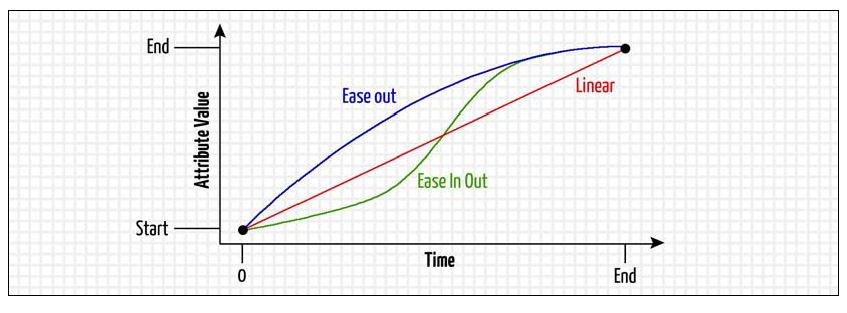
\includegraphics[width=0.7\linewidth]{obrazky/easing}
\caption{Graf troch easing typov}
\label{fig:easing}
\end{figure}


For each easing type, the rate at which the attribute changes varies along the graph in
the time axis. Each easing type can be described as such:
\begin{itemize}
	

\item Linear: The value varies consistently from its start value to its end value over
the course of the animation
\item Ease Out: The value increases quickly towards its end point before slowing
down towards the end of the animation
\item Ease In Out: The value decreases slowly at first and then increases quickly
before finally slowing down to its end point towards the end of the animation
\end{itemize}

\newpage
\clearpage
\begin{center}
	Prazdna strana
$vymaz$
\end{center}
\newpage
\clearpage


\subsection{Animácia transformácií}
TODO ASI TEN VENTIL BY BOLO VHODNE ZANIMOVAT A TRANSFORMOVAT

\subsection{Animacia vyuzivajuca vlastne atributy}
\subsection{Animacia podla path}
toto uz v prikladoch mam ako mapu TODO /
todo urobit pri nadrzi 

\subsection{Pausing a resuming animation}










%
%%\section{append()}
%%
%%\section{Element.attr(...)}
%%Vráti alebo nastaví dané atribúty elementu.
%%
%%\subsection{Parametre:}
%%\begin{itemize}
%%	\item objekt - obsahuje pár kľúč-hodnota atribútov, ktoré chcem nastaviť.
%%	\item string - názov atribútu
%%\end{itemize}
%% Niekoľko možných dvojíc parametrov sú v tabuľke \ref{parametre:attr}. Vráti buď súčasný element alebo stringovú hodnotu atribútu.
%%%
%%\subsection{
%%Použitie:}
%%\begin{lstlisting}
%%el.attr({
%%	fill: "#fc0",
%%	stroke: "#000",
%%	strokeWidth: 2, 
%%});
%%\end{lstlisting}
%
%
%\begin{table}[tp]
%	\begin{center}
%	
%	%\begin{tabular}{|l|p{3.9cm}|p{5.9cm}|}
%	\begin{tabular}{|l|p{4.5cm}|p{6.5cm}|}
%	\hline \textbf{Parameter} & \textbf{Príklad použitia} & \textbf{Poznámka} \\ 
%%		\hline cx & cx: 50 & x-os súradnica centra kruhu, alebo elipsy \\ 
%%		\hline cy & cy: 90 & y-os súradnica centra kruhu, alebo elipsy \\ 
%%		\hline r & r: 40 & polomer kruhu, elipsy alebo okruhlých rohov na obdĺžniku \\ 
%%		\hline rx & r: 50 & horizontálny polomer elipsy \\ 
%%		\hline ry & r: 40 & vertikálny polomer elipsy \\ 
%%		\hline x, y & x: 50, y: 100 & súradnica x-osi, y-osi  \\ 
%%			\hline width, height & width: 500, height: 10 & šírka, výška \\ 
%%			\hline "fill-opacity" & "fill-opacity": 0.5 & neprehľadnosť, 0-1 \\ 
%%		\hline fill & fill: "blue" & vyplnenie farbou, gradientom, obrázkom \\ 
%%		\hline stroke & stroke: "blue" & farba výplne okraja \\ 
%%		\hline strokeWidth & strokeWidth: 2 & šírka okraja v px, default je 1 \\ 
%%		\hline strokeLinecap & strokeLinecap: "butt" & ["butt", "square", "round"] \\ 
%%		\hline strokeLinejoin &  strokeLinejoin: "round" & ["bevel", "round", "miter"] \\ 
%		\hline viewBox & & napr. viewBox: [0, 0, 800, 600]
%		  \\ 
%%		\hline strokeDasharray &    strokeDasharray: "5 3" & pole čiarok, bodiek, pomlčiek \\ 
%		\hline font &   font: $"$20px Source Sans Pro, sans-serif$"$& zmena písma, rodiny písma, veľkosti v pixeloch, a weight \\ 
%		\hline transform & transform: "t" + [0, 5] +
%		"r" + 20 & t - zmena súradníc, r - otočenie \\ 
%%			\hline path & path: "M10,10 210,10" & SVG cesta \\ 
%			\hline text & text: "snap" & zmení text elementu \\ 
%		\hline 
%	\end{tabular} 
%	
%		\end{center}
%		\caption{Výber možných parametrov pre funkciu Element.atrr(...)}
%		\label{parametre:attr}
%\end{table}
%
%
%
%\section{Element.animate()}
% Snap.animation = function (attr, ms, easing, callback) 
%
%- attr (object) attributes of final destination
%- duration (number) duration of the animation, 
%
%in milliseconds
%- easing (function) \#optional one of easing 
%
%functions of @mina or custom one
%- callback (function) \#optional callback 
%
%function that fires when animation ends
%
%
%%\section{Gradinets, Path String, Colour Parsing}
%
%%\subsection{Gradients}
%%Sú dve možnosti ako zobraziť gradient.
%%\begin{itemize}
%%	\item \textbf{Lineárny gradientový formát: } $<$uhol$>$/$<$farba$>$[-$<$farba$>$[:$<$ofset$>$]]*-$<$farba$>$", napríklad: "90 - \#fff - \#000" - $90^o$ gradient z bielej na čiernu
%%	alebo "0 - \#fff - \#00f : 20 - \#000" $0^o$ gradient z bielej cez modrú pri  20\% a potom na čiernu. 
%%	\item \textbf{Radial gradient: }"r[($<$fx$>$, $<$fy$>$)]$<$farba$>$[-$<$farba$>$[>$<$ofset$>$]]*-$<$farba$>$", napríklad: "r\#fff-\#000" - je gradient z bielej na čiernu alebo "r(0.25, 0.75)\#fff-\#000" - gradient z bielej na čiernu s zameraním na bod 0.25 a 0.75. Súradnicové body sú zo škály 0...1. Môžu byť len použité pre kruhy, a elipsy.
%%\end{itemize}
%
%%
%%\subsection{Paper.path([pathString])}
%%Vytvorí $<$path$>$ element podľa daného reťazca. Parameter pozostáva z jedno písmenkových príkazov, nasledovanými bodkami a oddeľovaný argumentami a číslami. 
%%Napríklad: "M10,20L30,40" - obsahuje príkazy: M s argumentami (10, 20) a L (30, 40). Rozdiel vo veľkosti písma vyjadruje to, či ide o absolútnu, alebo relatívnu cestu. Ak sú malé znaky jedná sa o relatívne, v prípade veľkých znakov absolútna cesta. 
%%%\begin{center}
%%\begin{table}
%%\begin{center}
%%	\begin{tabular}{|c|c|c|}
%%	\hline \textbf{Príkaz} & \textbf{Názov} & \textbf{Parametre} \\
%%	\hline M & moveto & (x y)+ \\ 
%%	\hline Z & closepath & (none) \\ 
%%	\hline L & lineto & (x y)+ \\ 
%%	\hline H & horizonal lineto & x+ \\ 
%%	\hline V & vertical lineto & y+ \\ 
%%	\hline C & curveto & (x1 y1 x2 y2 x y)+ \\ 
%%	\hline S & smooth curveto & (x2 y2 x y)+ \\ 
%%	\hline Q & quadratic Bézier curveto & (x1 y1 x y)+ \\ 
%%	\hline T & smooth quadratic Bézier curveto & (x y)+ \\ 
%%	\hline 
%%\end{tabular} 
%%\end{center}
%%\caption{Niekoľko príkazov na tvorbu pathString}
%%\label{prikazyPath}
%%\end{table}
%%	\end{center}
%		
%
%
%
%%\section{Easing}
%%\begin{lstlisting}[language = HTML]
%%-	“linear”
%%- 	“<” or “easeIn” or “ease-in”
%%-	“>” or “easeOut” or “ease-out”
%%-	“<>” or “easeInOut” or “ease-in-out”
%%- 	“backIn” or “back-in”
%%- 	“backOut” or “back-out”
%%- 	“elastic”
%%- 	“bounce”
%%\end{lstlisting}
%
%%\begin{itemize}
%%\item 	“linear”
%%\item 	“<” or “easeIn” or “ease-in”
%%\item 	“>” or “easeOut” or “ease-out”
%%\item 	“<>” or “easeInOut” or “ease-in-out”
%%\item 	“backIn” or “back-in”
%%\item 	“backOut” or “back-out”
%%\item 	“elastic”
%%\item 	“bounce”
%%\end{itemize}
%
%
%
